\documentclass[border=10pt]{standalone}

\usepackage[utf8]{inputenc}                                 % Codificação do documento
\usepackage[T1]{fontenc}                                    % Seleção de código de fonte
\usepackage{microtype}                                      % Melhora a justificação do documento
\usepackage{lmodern}                                        % Usa a fonte Latin Modern
\usepackage{ae, aecompl}                                    % Fontes de alta qualidade

\usepackage{amsmath}
\usepackage{verbatim}
\usepackage{tikz}
\usetikzlibrary{arrows,calc,positioning,shadows.blur,decorations.pathreplacing}
\usepackage{etoolbox}

\usepackage{fontawesome}

\begin{document}
\begin{tikzpicture}
[
	              y = -1cm,
	           ->, >= stealth',
	  node distance = 2cm,
	  vertex/.style = { draw=black, circle, inner sep=2.5pt },
         dot/.style = { draw=black, fill=black, circle, inner sep=0.75pt },
	   label/.style = { draw=none, fill=none, anchor=west },
	toplabel/.style = { draw=none, fill=none, anchor=south }
]
    \node (Node)                at (7  ,0  )    [label]     {\faFolderOpen};
	\node (NodeLabel)           at (7.5,0  )    [label]     {\texttt{node}};
    \node[white] (VerticalLine) at (7  ,1.9)    [label]     {\faFolderOpen};
    \draw[-] (Node) edge[opacity=0.4] (VerticalLine);

        \node (Lib)                 at (7.5,0.5)    [label]     {\faFolderOpen};
	    \node (LibLabel)            at (8  ,0.5)    [label]     {\texttt{lib}};
        \node[white] (VerticalLine) at (7.5,1.9)    [label]     {\faFolderOpen};
	    \draw[-] (Lib) edge[opacity=0.4] (VerticalLine);

            \node (Fs)                  at (8  ,1  )    [label]     {\faFileText};
	        \node (FsLabel)             at (8.5,1  )    [label]     {\texttt{fs.js}};

            \node (Path)                at (8  ,1.5)    [label]     {\faFileText};
	        \node (PathLabel)           at (8.5,1.5)    [label]     {\texttt{path.js}};

	\node (Gulp)                at (0  ,0  )    [label]     {\faFolderOpen};
	\node (GulpLabel)           at (0.5,0  )    [label]     {\texttt{gulp}};
    \node[white] (VerticalLine) at (0  ,7.9)    [label]     {\faFolderOpen};
    \draw[-] (Gulp) edge[opacity=0.4] (VerticalLine);

        \node (NodeModules)         at (0.5,0.5)    [label]     {\faFolderOpen};
	    \node (NodeModulesLabel)    at (1  ,0.5)    [label]     {\texttt{node\_modules}};
        \node[white] (VerticalLine) at (0.5,3.4)    [label]     {\faFolderOpen};
	    \draw[-] (NodeModules) edge[opacity=0.4] (VerticalLine);

            \node (Deprecated)          at (1  ,1  )    [label]     {\faCube};
	        \node (DeprecatedLabel)     at (1.5,1  )    [label]     {\texttt{deprecated}};

            \node (GulpUtil)            at (1  ,1.5)    [label]     {\faCube};
	        \node (GulpUtilLabel)       at (1.5,1.5)    [label]     {\texttt{gulp-util}};

            \node (Orchestrator)        at (1  ,2  )    [label]     {\faCube};
	        \node (OrchestratorLabel)   at (1.5,2  )    [label]     {\texttt{orchestrator}};

            \node (Util)                at (1  ,2.5)    [label]     {\faCube};
	        \node (UtilLabel)           at (1.5,2.5)    [label]     {\texttt{util}};

            \node (Vinyl)               at (1  ,3  )    [label]     {\faCube};
	        \node (VinylLabel)          at (1.5,3  )    [label]     {\texttt{vinyl-fs}};

        \node (Lib)                 at (0.5,3.5)    [label]     {\faFolderOpen};
	    \node (LibLabel)            at (1  ,3.5)    [label]     {\texttt{lib}};
        \node[white] (VerticalLine) at (0.5,5.9)    [label]     {\faFolderOpen};
	    \draw[-] (Lib) edge[opacity=0.4] (VerticalLine);

            \node (Completion)          at (1  ,4  )    [label]     {\faFileText};
	        \node (CompletionLabel)     at (1.5,4  )    [label]     {\texttt{completion.js}};
            \node[white] (VerticalLine) at (1  ,4.9)    [label]     {\faFileText};
	        \draw[-] (Completion) edge[opacity=0.4] (VerticalLine);

                \node (AnonymousFunction)           at (1.5,4.5)    [label]     {\textit{fn}};
	            \node (AnonymousFunctionLabel)      at (2  ,4.5)    [label]     {\texttt{Anonymous Function}};

            \node (TaskTree)            at (1  ,5  )    [label]     {\faFileText};
	        \node (TaskTreeLabel)       at (1.5,5  )    [label]     {\texttt{taskTree.js}};
            \node[white] (VerticalLine) at (1  ,5.9)    [label]     {\faFileText};
	        \draw[-] (TaskTree) edge[opacity=0.4] (VerticalLine);

                \node (AnonymousFunction)           at (1.5,5.5)    [label]     {\textit{fn}};
	            \node (AnonymousFunctionLabel)      at (2  ,5.5)    [label]     {\texttt{Anonymous Function}};

        \node (Index)               at (0.5,6  )    [label]     {\faFileText};
	    \node (IndexLabel)          at (1  ,6  )    [label]     {\texttt{index.js}};
        \node[white] (VerticalLine) at (0.5,7.9)    [label]     {\faFileText};
	    \draw[-] (Index) edge[opacity=0.4] (VerticalLine);

            \node (Run)                 at (1  ,6.5)    [label]     {\textit{fn}};
	        \node (RunLabel)            at (1.5,6.5)    [label]     {\texttt{run}};

            \node (Watch)               at (1  ,7  )    [label]     {\textit{fn}};
	        \node (WatchLabel)          at (1.5,7  )    [label]     {\texttt{watch}};
            \node[white] (VerticalLine) at (1  ,7.9)    [label]     {\textit{fn}};
	        \draw[-] (Watch) edge[opacity=0.4] (VerticalLine);

                \node (AnonymousFunction)           at (1.5,7.5)    [label]     {\textit{fn}};
	            \node (AnonymousFunctionLabel)      at (2  ,7.5)    [label]     {\texttt{Anonymous Function}};

\end{tikzpicture}
\end{document}